%\vspace{1.5pc}
\vspace{1.5pc}
%\section[State of the Art]{State of the Art}
\begin{spacing}{1.5}
	
	Bab ini menjelaskan lebih detail mengenai pustaka relevan dan tinjauan teori dalam analisis laut lagrangian, persamaan yang mendasari, serta software yang digunakan dalam melakukan pelacakan sampah plastik di lautan. Hal ini bertujuan untuk mereview, mengupdate, mengkritik dan mensintesis literatur, melakukan meta-analisis literatur, melakukan konsepsi ulang dari topik yang direview, dan menjawab pertanyaan spesifik penelitian dari topik yang telah direview dalam literatur \shortcite{Torraco2016}. Struktur pembahasan studi relevan dan tinjauan teori selanjutnya dibagi dalam beberapa hal: pertama, akan dibahas mengenai persamaan gerak fluida dan Navier-Stokes dalam pemodelan laut secara umum, kedua tentang analisis laut lagrangian dan gaya yang berpengaruh, dan terakhir, akan dibahas mengenai histori penggunaan dari software Ocean\textbf{Parcels} dan grid yang digunakan. Terdapat banyak penelitan yang menggunakan software analisis laut lagrangian untuk mensimulasikan pergerakan air, plastik, plankton, dan ikan dengan berbagai macam gaya hidrodinamika. Meskipun demikian, karena fokus dari penelitian ini adalah pelacakan sampah plastik menggunakan software Ocean\textbf{Parcels} dengan gaya angin, hal ini tidak akan direview secara detail dan hanya akan dirujuk sebagaimana mestinya.
	
	
\end{spacing}
\vspace{-0.1pc}
\section[Persamaan Gerak Fluida]{Persamaan Gerak Fluida}
\begin{spacing}{1.5}
	
	Persamaan matematika yang mengatur aliran viskoelastik fluida berasal dari persamaan-persamaan hukum konservasi fisika yaitu konservasi massa, momentum dan persamaan konstitutif reologi \shortcite{Alves2021}. Penjabaran dari hukum-hukum tersebut menentukan bagaimana suatu persamaan model hidrodinamika dibuat. Salah satu persamaan fluida yang paling terkenal adalah persamaan Navier-Stokes yang terdiri dari persamaan momentum, persamaan kontinuitas, dan persamaan kekekalan densitas \shortcite{Haditiar2020}. Persamaan Navier-Stokes digunakan untuk menggambarkan fluida yang mengalir dan dianggap memiliki pergerakan yang kontinu. Diketahui bahwa hasil pengamatan dari sebuah partikel fluida yang mengalir memiliki sifat-sifat fluida secara umum yaitu kecepatan, temperatur, tekanan dan densitas \shortcite{Rafiq2019,Das2018,Khan2019}. Sebuah partikel fluida diilustrasikan pada Gambar \ref{fig:cube}a, dan \ref{fig:cube}b. Komponen fluida seperti tekanan $p$, kecepatan $u$, dan densitas $\rho$ terletak pada pusat partikel yang bergantung terhadap waktu $(t)$ dan ruang $(x,y,z)$. Sehingga, komponen-komponen tersebut dapat ditulis dalam fungsi $p(x,y,z,t), u(x,y,z,t)$  dan $\rho(x,y,z,t)$. 
	
	\begin{figure}[H]
		\centering
		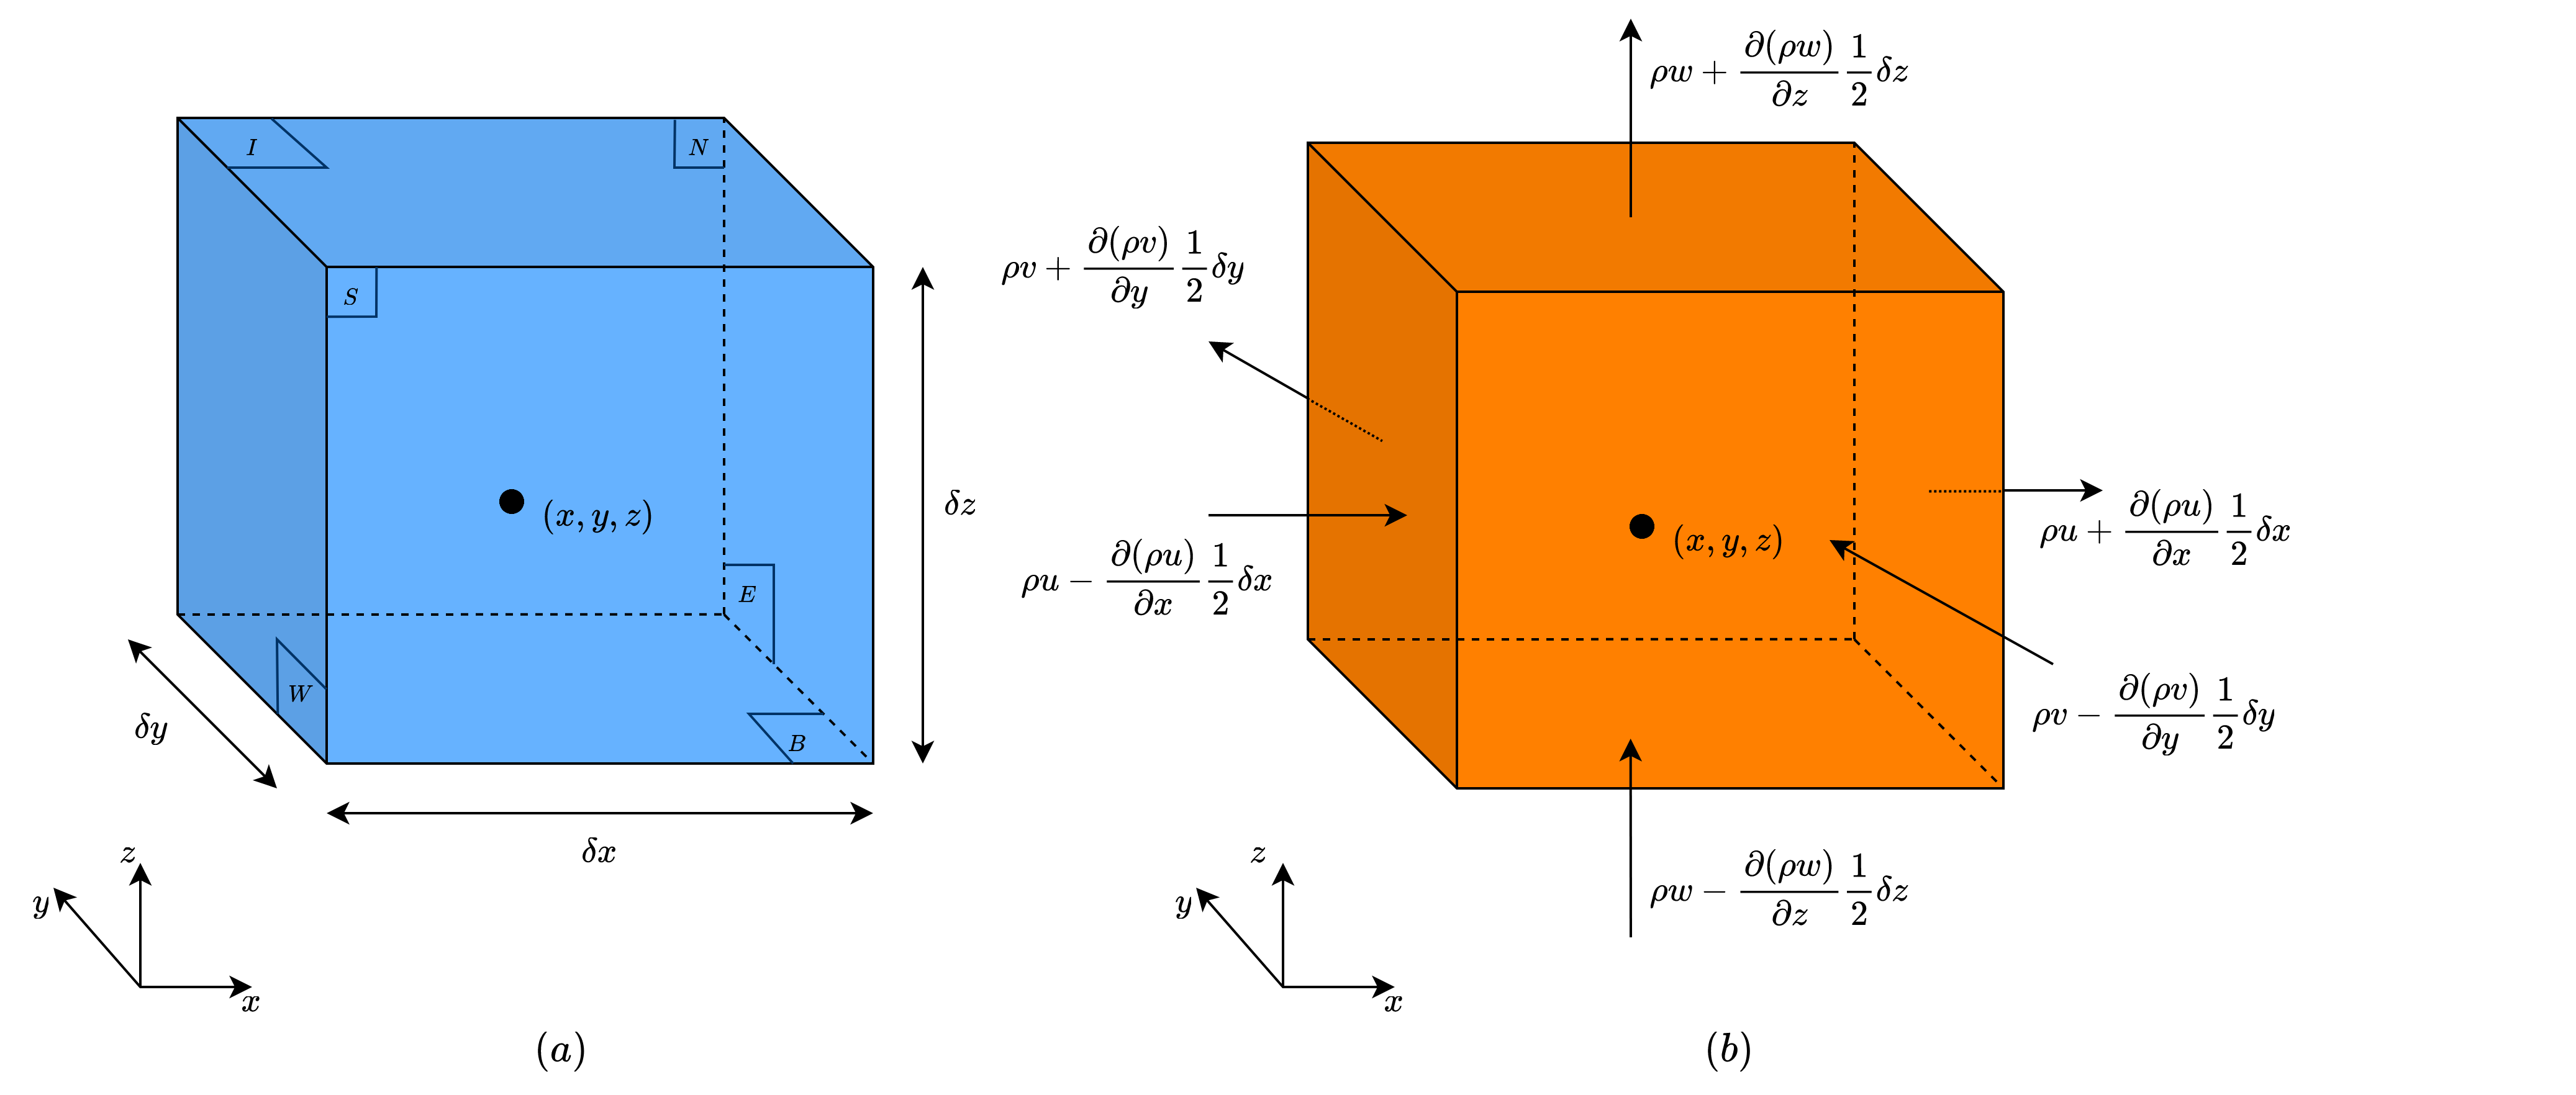
\includegraphics[width=16cm]{contents/cube}
		\caption{(a) Ilustrasi partikel sebagai sifat fisis fluida. (b) Aliran massa jenis masuk dan keluar \protect\shortcite{versteeg2007introduction}}
		\label{fig:cube}
		\medspace
		\small
		Massa jenis dari partikel $\rho(x,y,z,t)$ pada gambar bagian (a) dapat diterjemahkan sebagai aliran yang masuk dan keluar. Pada gambar bagian (b), arah aliran massa jenis pada partikel pusat merupakan jumlahan dari aliran massa jenis masuk dan keluar. Dengan cara yang sama, dapat juga dilakukan untuk tekanan dan kecepatan. 
	\end{figure}
	
\end{spacing}
\vspace{-1pc}
\section[Persamaan Navier-Stokes 3 Dimensi]{Persamaan Navier-Stokes 3 Dimensi}
\begin{spacing}{1.5}
	\par Model sirkulasi laut atau \textit{Ocean General Circulation Models} (OGCM) menggunakan persamaan Navier-Stokes untuk memodelkan fenomena fisis yang terjadi di lautan. Persamaan gerak Navier-Stokes nonhidrostatik dalam model 3-D terdiri dari persamaan momentum, persamaan kontinuitas, dan persamaan konservasi densitas \shortcite{Haditiar2020}. Pada model Navier-Stokes dengan pendekatan nonhidrostatik, tekanan air laut (P) dipecah menjadi dua bagian utama, yaitu: tekanan hidrostatik (p) dan tekanan nonhidrostatik (q)
	\begin{equation}
		P = p+q.
	\end{equation}
	Tekanan p dihitung secara diagnostik dari densitas  dan percepatan gravitasi g seperti pada persamaan berikut 
	\begin{equation}
		\frac{\partial p}{\partial z} = -(\rho - \rho_0)g.
	\end{equation}
	Sedangkan tekanan q dihitung secara prognostik dalam persamaan momentum (implisit). Hal ini karena tekanan q bergantung terhadap sirkulasi arus.
	\par Persamaan momentum lengkap untuk model nonhidrostatik adalah sebagai berikut
	\begin{equation}
		\begin{aligned}
			\frac{\partial u}{\partial t} + \text{adv}(u)-fv &= \frac{-1}{\rho_0}\frac{\partial(p+q)}{\partial x}+\text{diff}(u) \\
			\frac{\partial v}{\partial t} + \text{adv}(v)+fu &= \frac{-1}{\rho_0}\frac{\partial(p+q)}{\partial y}+\text{diff}(v) \\
			\frac{\partial w}{\partial t} +\text{adv}(w) &= \frac{-1}{\rho_0}\frac{\partial(q)}{\partial y}+\text{diff}(w).
		\end{aligned}	
	\end{equation}
	\par Dengan $\text{adv}(\psi)=u\frac{\partial \psi}{\partial x}+v\frac{\partial \psi}{\partial y}+w\frac{\partial \psi}{\partial z}$ adalah persamaan adveksi dan $\text{diff}(\psi)=\frac{\partial}{\partial x}(A_{H} \frac{\partial \psi}{\partial x})+\frac{\partial}{\partial y}(A_{H} \frac{\partial \psi}{\partial y})+\frac{\partial}{\partial z}(A_{Z} \frac{\partial \psi}{\partial z})$ adalah persamaan difusi dengan $A_H$ dan $A_Z$ koefisien gesekan eddy horizontal dan vertikal. 
	\par Kecepatan arus dalam sistem koordinat Cartesian 3-D didefinisikan dengan u,v, dan w. Waktu didefinisikan dengan t, parameter Coriolis dengan f, dan densitas air laut referensi dengan $\rho_0$.
	Untuk persamaan kontinuitas atau kekekalan volume diekspresikan dalam persamaan berikut
	\begin{equation}
		\frac{\partial u}{\partial t} + \frac{\partial v}{\partial t} + \frac{\partial w}{\partial t} = 0.
	\end{equation}
	Berdasarkan persamaan kontinuitas (2.4), tekanan dinamis pada lapisan permukaan dapat dihitung dengan persamaan berikut
	\begin{equation}
		\frac{\partial q_s}{\partial t} = \rho_0 g_i \times \left( \frac{(\partial \left(H \langle u \rangle \right)} {\partial x} + \frac{(\partial \left(H \langle v \rangle \right)} {\partial y}\right)
	\end{equation}
	dengan $q_s = \rho_0 g \eta$. Disini $\rho_0$ adalah densitas air laut referensi, dan $\eta$ adalah elevasi permukaan laut, $H$ adalah total kedalaman laut, dan $< >$ adalah operator rata-rata vertikal.
	\par Densitas air laut bergantung pada temperatur, salinitas, dan tekanan. Selanjutnya asumsikan bahwa air laut hanya bergantung linear terhadap temperatur dan salinitas, serta difusifitas \textit{eddy} untuk temperatur dan salinitas sama. Persamaan konservasi densitas diberikan oleh,
	\begin{equation}
		\frac{\partial \rho}{\partial t} + \text{adv}(\rho) = \text{diff}(\rho).
	\end{equation}
	Dalam aplikasinya, persamaan Navier-Stokes tidak hanya digunakan untuk memodelkan laut, tapi juga merambah ke bidang pemodelan cuaca \shortcite{Rohli2021}, aliran air dalam pipa \shortcite{Ouchiha2012} dan aliran udara di sekitar sayap pesawat \shortcite{Tulus2019}. Dalam bentuk persamaan lengkap dan simplifikasi, persamaan ini juga dapat digunakan untuk mendesain kereta api \shortcite{Croquer2020}, pesawat terbang \shortcite{Chau2021}, dan mobil \shortcite{Ambarita2018}. Terdapat juga studi tentang aliran darah \shortcite{Gill2021}, desain stasiun pembangkit listrik \shortcite{Yang2019}, dan analisis polusi udara \shortcite{Issakhov2022}. 
\end{spacing}
\vspace{-0.1pc}
\section[Analisis Laut Lagrangian]{Analisis Laut Lagrangian}
\begin{spacing}{1.5}
	\justifying
	\par Pergerakan partikel plastik tidak terlepas dari pergerakan air di laut (fluida). Secara umum, terdapat 2 konsep atau kerangka dasar yang digunakan untuk mensimulasikan pergerakan air di lautan yaitu pendekatan Lagrangian dan pendekatan Eulerian. Dalam pendekatan Lagrangian, pergerakan tiap partikel dinyatakan dan diobservasi sebagai fungsi waktu dan dianggap bahwa kerangka acuan bergerak bersama-sama dengan partikel fluida. Dalam hal ini posisi, kecepatan dan percepatan tiap-tiap partikel fluida dapat dinyatakan sebagai $s(x_0,y_0,z_0,t), V(x_0,y_0,z_0,t), \;\text{dan}\; a(x_0,y_0,z_0,t) \;\text{dengan}\; (x_0,y_0,z_0)$ adalah posisi awal partikel. Sedangkan dalam pendekatan Eulerian, pergerakan tiap partikel dinyatakan dan diobservasi sebagai fungsi ruang dan waktu dengan kerangka acuan tetap. Kecepatan fluida dinotasikan sebagai $V = V(x,y,z,t)$. Lebih lanjut, dapat diobservasi laju perubahan kecepatan yang melewati titik observasi dan berubah terhadap waktu yaitu, $\frac{\partial V}{\partial x}, \frac{\partial V}{\partial y}, \frac{\partial V}{\partial z}, \;\text{dan}\;\frac{\partial V}{\partial t}$ \shortcite{Potter2010}.
	\par Dari pendekatan diatas, keduanya memiliki kelebihan maupun kekurangan. Pendekatan Lagrangian memungkinkan penyimpanan dan analisis lintasan dari partikel, akan tetapi kelemahannya adalah lebih sulit dalam menghitung jumlah agregat partikel. Sebaliknya, pendekatan Eulerian lebih mudah dalam menghitung evolusi konsentrasi partikel sepanjang waktu tapi terbatas dalam melihat riwayat lintasan partikel. Secara umum, tujuan teknis dari analisis laut Lagrangian adalah untuk memperkirakan lintasan partikel virtual fluida dengan memanfaatkan informasi Eulerian fluida, yaitu medan kecepatan \shortcite{VanSebille2018}. Selanjutnya akan dijabarkan mengenai teori kinematik dan algoritma komputasi yang berkaitan dengan kedua pendekatan ini.
	\par Asumsikan terdapat titik partikel dimana vektor posisi dari partikel $X(t)$ bergantung terhadap waktu $t$. Kurva dalam ruang dalam hal ini dapat dideskripsikan sebagai lintasan dari partikel. Partikel diasumsikan dapat memiliki bentuk diskrit dan kontinu. \textsc{Apabila terdapat sejumlah $n$ buah partikel diskrit ($n \in \mathbb{N}$), vektor posisi dari partikel-partikel ini dapat dikombinasikan dan dinotasikan sebagai $X^n(t)$, dan apabila partikel memiliki bentuk kontinu,} $n$ disini menjadi label kontinu, dan pergerakan partikel dalam bentuk ini dinotasikan sebagai $x=X(a,t)$ dimana $a$ adalah koordinat materi, posisi partikel dengan referensi waktu $t=t_0$.
	\par Kumpulan molekul dalam skala mikroskopik disebut sebagai parsel fluida (\textit{fluid parcel}). Kecepatan parsel fluida didefinisikan sebagai rata-rata tertimbang massa dari kecepatan masing-masing molekul. Dalam bentuk kontinu, parsel fluida dianggap memiliki volume materi berukuran kecil dan kecepatan parsel fluida dapat dicari dengan menghitung turunan lintasan partikel terhadap waktu (koordinat materi $a$ dianggap konstan),
	\begin{equation}\label{eq:basic_traj}
		v(x,t) = \left(\frac{\partial X(a,t)}{\partial t}\right)_a
	\end{equation}
	dengan $v$ adalah kecepatan partikel dan $x = X(a,t)$. Perhatikan bahwa persamaan ini adalah persamaan matematis yang menghubungkan pendekatan Lagrangian dan Eulerian dengan cara menyamakan kecepatan partikel yang melintasi suatu titik dalam ruang $x=X(a,t)$ dengan medan kecepatan fluida di titik tersebut.
	\par Lebih lanjut, untuk memperoleh deskripsi kinematik yang lebih lengkap, diperkenalkan fungsi sembarang $\psi$ yang dihitung disepanjang lintasan, $\psi(X(a,t),t)$. Dengan menggunakan aturan rantai diperoleh,
	\begin{equation*}
		\begin{aligned}
		\frac{\partial \psi(X(a,t),t)}{\partial t}&=\frac{\partial \psi(X(a,t),t)}{\partial t} + \left(\frac{dX(a,t)}{dt}\right)\frac{\partial \psi(X(a,t),t)}{\partial X(a,t)}  \\
		&= \left[\frac{\partial}{\partial t} + v(X(a,t),t)\frac{\partial}{\partial X(a,t)}\right]\psi(X(a,t),t),
		\end{aligned}
	\end{equation*}
	atau secara umum diperoleh,
	\begin{equation}
		\frac{\partial \psi(X(a,t),t)}{\partial t}=\left[\frac{\partial}{\partial t}+v(X(a,t),t).\nabla\right]\psi(X(a,t),t).
	\end{equation}
	Saat lintasan diabaikan (pendekatan Eulerian), diperoleh persamaan yang lebih ringkas untuk turunan materi terhadap waktu
	\begin{equation}
		\frac{D \psi(x,t)}{D t}=\left[\frac{\partial}{\partial t}+v(x,t).\nabla\right]\psi(x,t).
	\end{equation}
	\par Simbol $D$ digunakan untuk membedakan antara turunan materi terhadap waktu dengan turunan waktu yang lebih umum yang tidak mensyaratkan harus diikuti oleh partikel materi fluida. Sehingga apabila, $x=\psi(x,t)$, turunan materi terhadap waktu diberikan oleh medan kecepatan dititik tersebut
	\begin{equation*}
		\frac{Dx}{Dt}=v(x,t).
	\end{equation*}
	\par Saat menggunakan model laut, terdapat dua metode yang digunakan untuk mengintegrasi Lagrangian. Metode yang pertama terjadi secara online, dimana lintasan dihitung disetiap langkah waktu sehingga model Eulerian diperbaharui secara terus-menerus. Metode yang kedua terjadi secara offline dan memanfaatkan sampel medan kecepatan yang tersimpan dari model Eulerian. Perhitungan model offline menawarkan kemampuan untuk menghitung lintasan dalam mode maju (dari titik awal dan maju dalam waktu) atau dalam mode mundur (dari titik akhir dan mundur dalam waktu)\shortcite{VanSebille2018}.
	\par Untuk menganalisis lintasan partikel terdapat beberapa software yang dapat digunakan dan tentunya memiliki kelebihan dan kekurangan masing-masing. Software ini ditulis dengan beragam bahasa seperti Python, Fortran, GNU/Octave, dan C++. Diantara software yang menghitung Lagrangian secara offline adalah \href{https://www.univ-brest.fr/lpo/ariane}{Ariane}, \href{tracmass.org}{TRACMASS}, \href{https://github.com/jinbow/Octopus}{Octopus}, \href{https://bitbucket.org/f_nencio/spasso/overview}{LAMTA}, \href{https://github.com/beatrixparis/connectivity-modeling-system}{CMS}, dan \href{oceanparcels.org}{Parcels}. Dalam perhitungan online, software yang dapat digunakan adalah \href{mpas-dev.github.io}{LIGHT in MPAS-O}, \href{nemo-ocean.eu/About-NEMO/Reference-manuals}{NEMO online floats and icebergs}, \href{mitgcm.org}{MITgcm}, \href{hycom.org}{HYCOM Float Package}, dan \href{myroms.org/wiki/floats.in}{ROMS online floats}. Selain dari perbedaan bahasa, perbedaan lainnya dapat dilihat dari data OGCM yang didukung, metode adveksi dan difusi, serta grid yang didukung \shortcite{VanSebille2018}.
	\par Terdapat beberapa proses transportasi dilautan yang mempengaruhi pergerakan dari partikel plastik, diantaranya adalah pengaruh daya apung (\textit{stokes drift}) dan angin.
\subsection[Pengaruh Stokes Drift]{Pengaruh Stokes Drift}
	Kecepatan stokes drift secara umum didefinisikan sebagai selisih antara rata-rata kecepatan Lagrangian dari parsel fluida dengan rata-rata kecepatan arus Eulerian yang diukur pada titik tetap dalam ruang \shortcite{Monismith2020}. Dalam hal ini, jika diambil rata-rata masing-masing kecepatan dalam suatu periode waktu tertentu, sebagai contoh periode gelombang, maka diperoleh stokes drift $\overline{u_s}$ adalah
	\begin{equation}
		\overline{u_s}=\overline{u_L}-\overline{u_E},
	\end{equation}
	dengan $\overline{u_E},\overline{u_L}$ menyatakan rata-rata kecepatan Eulerian dan Lagrangian, dan
	\begin{equation*}
		\begin{cases}
			\overline{u_E} &= \overline{\frac{\partial x}{\partial t}} = \overline{u(x,t)}, \\
			\overline{u_L} &= \overline{\frac{\partial X(a,t)}{\partial t}} = \overline{u(X(a,t),t)}.
		\end{cases}	
	\end{equation*}
	\par Dikarenakan gaya stokes drift, partikel plastik yang terapung dilautan akan memiliki kecepatan dalam arah yang sama dengan perambatan gelombang. Gelombang yang dimaksud adalah gelombang gravitasi permukaan yang muncul dari antarmuka atmosfer dan laut \shortcite{Brach2018}. Secara umum, sangat sulit untuk mengetahui pengaruh stokes drift terhadap partikel serta hubungannya dengan mekanisme transportasi lain \shortcite{VanSebille2020} ditambah stokes drift tidak mempengaruhi akumulasi mikroplastik dalam skala besar tetapi meskipun demikian stokes drift berperan dalam peningkatan transportasi mikroplastik \shortcite{Onink2019,Iwasaki2017}.
\subsection[Pengaruh Angin]{Pengaruh Angin}
	Angin memainkan peran penting dalam mendorong arus permukaan dan juga dalam proses interaksi udara-laut. Sampah mikroplastik dapat ditransportasikan secara langsung oleh gaya angin dan mempengaruhi setiap benda yang berada diatas permukaan air \shortcite{VanSebille2020}. Sebagian besar proses interaksi udara-laut ditentukan dengan menggunakan tekanan angin (\textit{wind stress}), suatu ukuran transfer momentum yang disebabkan oleh gerakan relatif antara laut dan atmosfer \shortcite{Chacko2022}. Tekanan angin berdasarkan aerodinamis massal (\textit{bulk-aerodynamic}) dirumuskan sebagai,
	\begin{equation}
		\tau = \rho_a C_d U_w^2
	\end{equation}
	dengan $\rho_a$ adalah densitas udara $(1.225 kg/m^3)$, $C_d$ koefisien seret (\textit{dimensionless}) $(\approx 1.3 \times 10^-3)$ dan $U_w$ kecepatan angin.
\end{spacing}
\vspace{-0.1pc}
\section[OceanParcels]{OceanParcels}
\begin{spacing}{1.5}
	\justifying
	Ocean\textbf{Parcels} (\textbf{P}robably \textbf{A} \textbf{R}eally \textbf{C}omputationally \textbf{E}fficient \textbf{L}agrangian \textbf{S}imulator) adalah kumpulan \textit{class} dan \textit{method} dalam Python untuk membuat simulasi pelacakan partikel yang dapat disesuaikan menggunakan data output dari model sirkulasi laut (\textit{Ocean General Circulation Models} (OGCMs)) seperti NEMO \shortcite{Delandmeter2019,Wichmann2019}, HYCOM \shortcite{Onink2021,VanderMheen2020}, dan MITgcm \shortcite{Reijnders2022,Shakespeare2021}. Parcels dapat digunakan untuk melacak partikel-partikel yang aktif dan pasif seperti air, plankton, plastik, dan ikan. Dalam hal ini, partikel dalam Parcels merepresentasikan berbagai benda yang mengapung dan tenggelam di lautan (\href{https://oceanparcels.org/}{https://oceanparcels.org/}, \shortciteA{Lange2017}).
	\par Pertama kali dikembangkan pada tahun 2017, Ocean\textbf{Parcels} bertujuan untuk mengatasi masalah penggunaan software analisis laut Lagrangian yang tidak cukup dinamis dalam merespon peningkatan kompleksitas, skala, dan kebutuhan untuk kostumisasi kasus penggunaan \shortcite{Lange2017}. Beberapa project telah menggunakan framework Parcel untuk mensimulasikan plankton yang tenggelam di lautan (\href{https://planktondrift.science.uu.nl/}{planktondrift.org}), transportasi mikroba di lautan (\href{https://adrift-project.com/}{Adrift project}), serta \href{http://topios.org/}{TOPIOS project} untuk membuat peta 3D dari polusi plastik di lautan. Dalam projek \href{https://planktondrift.science.uu.nl/}{planktondrift.org}, transportasi mikroplankton - atau dinoflagellate cyst (dinocyst) - dimodelkan dalam model global resolusi tinggi ($0.1^\circ$ secara horizontal) dengan mempertimbangkan arus 3D, dan kecepatan tenggelam partikel per hari dan membandingkan kondisi laut dalam simulasi partikel sedimen asal dengan air di atas permukaan laut secara langsung \shortcite{Nooteboom2019}. Temuan dari simulasi mikroplankton menunjukkan bahwa terdapat perbedaan hasil signifikan dalam simulasi dengan data OGCM yang menggunakan eddies dan non-eddies \shortcite{Nooteboom2020}. 
	\par Model simulasi mikroba dalam \href{https://adrift-project.com/}{Adrift project} menunjukkan bahwa terdapat pola yang berbeda dalam toleransi termal fototrof mikroba dari massa air yang berdekatan yang diambil sampelnya di Samudra Pasifik barat daya, ditentukan menggunakan penanda fluoresen untuk spesies oksigen reaktif (ROS). Eksperimen dilakukan dengan mempertimbangkan data arus, dan temperatur dari model OGCM. Studi dengan jelas menunjukkan bahwa divergensi fenotipik terjadi di sepanjang lintasan drift planktonik \shortcite{McInnes2019}.
	\par Sebaran partikel di lautan secara global dapat dilihat dalam gambar \ref{fig:partikel}. Gambar \ref{fig:partikel} di plot dengan menggunakan data partikel dari model NEMO dengan titik sentral wilayah perairan Indonesia.
	
	\begin{figure}[H]
		\centering
		\includegraphics[width=5cm]{contents/parcels.jpg}
		\caption{Partikel virtual di lautan global}
		\label{fig:partikel}
		\medskip
		\small
		Gambar direproduksi ulang dari \href{https://oceanparcels.org/}{https://oceanparcels.org/} dengan mengubah titik sentral wilayah perairan Indonesia
	\end{figure}
	\par Selain data output kecepatan dari model OGCM, Parcel dapat menggunakan data observasi dari \textit{floats} atau \textit{drifters} yang menghasilkan data kecepatan permukaan 2-D dan kecepatan geostropik permukaan \shortcite{VanSebille2018}. Selanjutnya perhatikan bahwa untuk menghitung lintasan partikel menggunakan medan kecepatan membutuhkan 2 hal, yaitu integrasi lintasan pada persamaan \ref{eq:basic_traj} dan interpolasi grid medan kecepatan dalam ruang dan waktu. 
	\par Apabila terdapat $n$ buah partikel yang berlokasi di titik $x=X^{(n)}(t)$, posisi dari partikel dapat diperbaharui dengan mengintegralkan persamaan \ref{eq:basic_traj} dan mengambil langkah waktu kecepatan sehingga
	\begin{equation}\label{eq:traj}
		X(t+\Delta t) = X(t)+\int_{t}^{t+\Delta t}v(x(\tau),\tau)d\tau + \Delta X_b(t),
	\end{equation}
	dengan $\Delta X_b(t)$ adalah tambahan suku di ruas kanan yang merepresentasikan perilaku partikel, seperti contoh daya apung (\textit{buoyancy}) \shortcite{VanSebille2018}. Solusi dari persamaan ini kemudian diaproksimasi dalam Parcels dengan langkah waktu numerik.
	\par Gambar \ref{fig:parcelsflowchart} menunjukan diagram alir dari Parcels. User atau pengguna dalam hal ini harus mendefinisikan variabel dari sistem, Partikel-partikel yang akan disimulasikan, dan rutinitas komputasi selain dari adveksi waktu (\textit{time advection}) yang disebut juga sebagai \textit{kernel}. Kemudian, algoritma Parcels akan melakukan perulangan untuk waktu yang terintegrasi dan memperbaharui kondisi partikel-partikel, mengapdatasi data \textit{field} OGCM yang dibutuhkan dan menghasilkan output. Output dari Parcels (dapat berupa \textit{NumPy array file} dalam format .npy atau berupa \textit{NetCDF file} dengan format .nc) selanjutnya dapat divisualisasikan secara \textit{real time}, yaitu simulasi pergerakan partikel, dan variasi temporal dari kecepatan atau properti lainnya.

	\begin{figure}[H]
		\centering
		\includegraphics[width=13cm]{contents/parcels_flowchart.png}
		\caption{Flowchart Parcels. Kode disusun dalam tingkat abstraksi tinggi, meminta dari pengguna informasi input yang sangat diperlukan \protect\shortcite{Lange2017}}.
		\label{fig:parcelsflowchart}
	\end{figure}
	\par Penerapan Ocean\textbf{Parcels} tidak terbatas pada simulasi plankton dan mikroba. Dengan mengkombinasikan model pelacakan partikel dengan data in situ perilaku tukik (anak penyu), dapat di simulasikan penyebaran penyu Neonatus di Samudera Hindia barat daya sekaligus mengetahui probabilitas kelangsungan hidup tukik \shortcite{LeGouvello2020}. Transportasi berbagai spesies ikan juga dapat disimulasikan dengan Parcel, diantaranya adalah ikan karang (Reel fish) di Kepulauan Hawaii dalam hubungannya dengan fenomena eddies yang tinggi \shortcite{Phillips2019}, simulasi ikan bentik kecil (Tripterygion tripteronotum) di laut Adriatik \cite{Sefc2020}, dan simulasi larva Pomatomus saltatrix (bluefish) untuk mengetahui persebaran dan mengidentifikasi kontribusi peristiwa pemijahan yang berbeda terhadap penyelesaian. Hal ini dilakukan dengan memodelkan penyebaran larva yang dilepaskan di wilayah utara dan lintang tengah selama musim semi dan musim panas Austral \shortcite{Schilling2020}.
	\par Simulasi sampah plastik di perairan global dengan menggunakan Parcel telah banyak dilakukan. Dalam penelitiannya, \citeNP{McAdam2018} menganalisis kesalahan yang melekat dengan pemetaan lintasan ke grid dan konsekuensi untuk pemodelan transportasi laut dan deteksi struktur akumulasi. Analisis sensitivitas dari parameter Rantai Markov dilakukan dalam pilin Stommel (\textit{Stommel gyre}) ideal dan arus batas barat serta dengan drifter laut yang diamati. Diketahui bahwa, aplikasi pendekatan rantai Markov dalam oseanografi mampu memodelkan pelacakan puing-puing plastik yang mengambang dan massa air secara global dan pada skala waktu tahunan hingga seratus tahun. Penelitian ini dilakukan dengan menfokuskan pada dua wilayah utama pertukaran antar laut - sistem Agulhas dan Atlantik utara. 
	\par Dalam penelitian lainnya, mikroplastik yang mengambang disimulasikan dengan menggunakan pelacakan partikel Lagrangian di perairan Atlantik utara, dan Pasifik utara dengan mempertimbangkan peran berbagai proses fisik, seperti Ekman permukaan dan arus geostropik, Stokes drift permukaan dan aktivitas eddy skala meso \shortcite{Onink2019}. Dalam memahami konsentrasi, karakteristik, dan dampak di lautan, simulasi di perairan permukaan samudera di Semenanjung Antartika dilakukan dengan mengukur dan mengkarakterisasi puing-puing plastik. Pengambilan sampel dilakukan melalui pukat-hela (\textit{surface trawl}) dan rata-rata konsentrasi sampah diperkirakan mencapai 1.794 $\text{item.km}^{-2}$ dengan berat rata-rata 27,8 $\text{g.km}^{-2}$ \shortcite{Lacerda2019}. Di tempat lainnya, penelitian dilakukan di samudera Hindia selatan untuk menentukan dinamika tambalan sampah dengan kedalaman dan mekanisme transportasi yang berbeda seperti arus permukaan laut, Stokes drift dan gaya angin secara langsung \shortcite{VanDerMheen2019}.
	\par Di wilayah Indonesia sendiri, telah dilakukan simulasi pelacakan sampah plastik dengan cara pelacakan  maju dan mundur di teluk Jakarta. Hal ini dilakukan untuk memahami jalur sampah laut di lautan dan mengidentifikasi strategi mitigasi sampah plastik \shortcite{Iskandar2021}. Selain itu, dari hasil simulasi pelacakan, sampah plastik yang berasal dari Indonesia bersama-sama dengan negara India, dan Filipina menyumbang 43.5\% dari total 48,304 ton sampah plastik yang terdampar di pantai Kenya \shortcite{Chassignet2021}.     
	
\subsection[Time Stepping]{Time Stepping}
	Persamaan \ref{eq:basic_traj} dan kondisi awal dapat ditulis ulang sebagai 
	\begin{equation}\label{eq:newbasic_traj}
		\dot y(t) = f(t,y(t)), \quad y(t_0)=y_0
	\end{equation}
	dengan posisi partikel pada waktu $t_n$ diberikan  oleh $y(t_n)=(x_n,y_n,z_n)$. Fungsi $f$ adalah kecepatan ($v$) dari partikel yang berbentuk suatu vektor (setiap elemen dalam $f$ adalah kecepatan dalam 1-D). Akibatnya persamaan \ref{eq:traj} (tanpa suku tambahan) menjadi
	\begin{equation}
		y(y_0,t+\Delta t) = y(y_0,t)+\int_{t}^{t+\Delta t}v(y,\tau)d\tau.
	\end{equation}
	\par Persamaan \ref{eq:newbasic_traj} dapat digunakan untuk mengaproksimasi posisi partikel pada waktu $t_{n+1}=t_n+h$, dengan $h$ adalah langkah waktu. Selanjutnya akan dijelaskan beberapa metode yang digunakan untuk melakukan hal ini. Metode yang paling mudah dan sering digunakan adalah metode eksplisit Euler. $f$ dalam hal ini didekati dengan $\textit{forward difference}$,
	\begin{equation*}
		f(t,y_n)=\dot y_n \approx \frac{y_{n+1}-y_n}{h},
	\end{equation*}
	sehingga solusi $y$ pada waktu $t+h$ menjadi
	\begin{equation}
		y_{n+1}=y_n+hf(t_n,y_n).
	\end{equation}
	Akurasi dari metode eksplisit Euler dapat ditingkatkan dengan mengambil turunan dari titik tengah,
	\begin{equation*}
		y_{n+1}=y_n+hf(t_{n+\frac{1}{2}},y_{n+\frac{1}{2}})
	\end{equation*}
	dimana nilai $y_{n+\frac{1}{2}}$ ditentukan dengan cara
	\begin{equation*}
		\begin{aligned}
			k_1 &= f(t_n,y_n) \\
			k_2 &= f(t_n+\frac{h}{2},y_n+\frac{h}{2}k_1) \\
			y_{n+1}&=y_n+hk_2.
		\end{aligned}
	\end{equation*}
	Apabila persamaan terakhir diperumum maka diperoleh metode eksplisit Runge-Kutta untuk $s$-tingkat yaitu,
	\begin{equation}\label{eq:RKN}
		\begin{aligned}
			k_1 &= f(t_n,y_n) \\
			k_2 &= f(t_n+c_2h,y_n+ha_{21}k_1) \\
			k_3 &= f(t_n+c_3h,y_n+h(a_{31}k_1+a_{32}k_2)) \\
			\vdots \\
			k_s &= f(t_n+c_sh,y_n+h(a_{s1}k_1+\cdots +a_{s(s-1)}k_{s-1})) \\
			y_{n+1}&=y_n+h(k_1+\cdots+b_sk_s).
		\end{aligned}
	\end{equation}
	Dalam \textit{Butcher tableau} \shortcite{Vermeire2019}, persamaan ini dapat dituliskan menjadi 
	\[
	\renewcommand\arraystretch{1.2}
	\begin{array}
		{c|ccccc}
		0\\
		c_2 & a_{21}\\
		c_3 & a_{31} & a_{32} \\
		\vdots& \vdots& \vdots& \ddots \\
		c_s & a_{s1} & a_{s2} & \cdots & a_{s(s-1)} \\
		\hline
		& b_1 & b_2 & \cdots & b_{s-1} & b_s
	\end{array}
	\]
	Selanjutnya perhatikan bahwa metode eksplisit Runge-Kutta Orde 4 (RK4) adalah kasus khusus dari Runge-Kutta untuk $s$-tingkat dan diformulasikan dalam $\textit{Butcher tableau}$ sebagai,
	\[
	\renewcommand\arraystretch{1.2}
	\begin{array}
		{c|cccc}
		0\\
		\frac{1}{2} & \frac{1}{2}\\
		\frac{1}{2} &0 &\frac{1}{2} \\
		1& 0& 0& 1\\
		\hline
		& \frac{1}{6} &\frac{1}{3} &\frac{1}{3} &\frac{1}{6} 
	\end{array}
	\]
	Karena time step $h$ dalam RK4 tetap maka untuk menghasilkan hasil aproksimasi yang lebih akurat diperlukan $h$ yang relatif kecil. Akibatnya adalah waktu komputasi yang digunakan akan semakin lama untuk menghasilkan solusi yang lebih baik. Hal ini mendasari penggunaan dari metode Runge-Kutta-Fehlberg (RKF45) yang merupakan pengembangan dari RK4. Dalam RKF45, orde ke 4 (5-tingkat) dan ke 5 (6-tingkat) dari persamaan \ref{eq:RKN} dihitung. Lebih lanjut, RKF45 dalam $\textit{Butcher tableu}$ direpresentasikan dalam bentuk,
	\[
	\renewcommand\arraystretch{1.2}
	\begin{array}
		{c|cccccc}
		0\\
		\frac{1}{4} & \frac{1}{4}\\
		\frac{3}{8} &\frac{3}{32} &\frac{9}{32} \\
		\frac{12}{13} &\frac{1932}{2197} & -\frac{7200}{2197} & \frac{7296}{2197}\\
		1 &\frac{439}{216} & -8 & \frac{3680}{513} & -\frac{845}{4104}\\
		\frac{1}{2} &-\frac{8}{27} & 2 & -\frac{3544}{2565} & \frac{1859}{4104} & -\frac{11}{40}\\
		\hline
		& \frac{16}{135} &0 &\frac{6656}{12825} &\frac{28561}{56430} & -\frac{9}{50} & \frac{2}{55} \\
		& \frac{25}{216} &0 &\frac{1408}{2565} &\frac{2197}{4104} & -\frac{1}{5} & 0
	\end{array}
	\]
	Baris bawah pertama dan kedua dalam tabel di atas merepresentasikan orde ke 5 dan orde ke 4 dari Runge-Kutta $s$-tingkat. Selisih antara orde ke 5 (RK5) dan orde ke 4 (RK4), dihitung dengan cara
	\begin{equation*}
		\kappa = || y_{n+1}^{5th}-y_{n+1}^{4th} ||.
	\end{equation*}
	Persamaan ini digunakan untuk menghitung $\textit{local error}$ di titik $n+1$.
	\par Ketiga metode yang sudah dijelaskan di atas telah diimplementasikan dalam Parcels dalam bentuk module: \textit{AdvectionEE,\; AdvectionRK4,\; AdvectionRK\_3D} dan \textit{AdvectionRK45} sehingga pengguna hanya perlu memanggil modul yang ada untuk melihat atau membandingkan lintasan dari partikel sesuai dengan metode numerik yang digunakan.
\subsection[Kondisi Batas]{Kondisi Batas}
	Saat menjalankan simulasi partikel, terdapat beberapa kondisi batas yang harus dipertimbangkan. Dalam bidang 2-D, terdapat kondisi batas antara darat dan laut serta sisi tepi dari domain simulasi yang digunakan. Dalam ruang 3-D, terdapat kedalaman lautan yang mempengaruhi sehingga kondisi batas yang berhubungan adalah antara laut dan dasar laut, atau laut dan permukaan laut. Terdapat beberapa kondisi berbeda yang mempengaruhi hal ini tergantung pada eksperimen yang dilakukan. Sebagai contoh, simulasi partikel yang berbeda bisa saja memiliki perilaku yang berbeda ketika mendekati tepi daratan. Partikel plastik dapat dibiarkan tersangkut (\textit{get stuck}) di pantai atau darat tapi hal ini tidak boleh terjadi apabila partikel yang disimulasikan adalah ikan atau biota laut lainnya. Dalam penelitian ini, kondisi batas yang digunakan adalah antara darat dan laut serta sisi tepi dari domain simulasi dan hanya membatasi pada kasus 2-D. 
\end{spacing}
\vspace{-0.3cm}
\section[Arakawa C-grid]{Arakawa C-grid}
\begin{spacing}{1.5}
	\justifying
	Data hidrodinamik atau output model OGCM disimpan sebagai kumpulan \textit{Fields} dalam Parcels yang memuat data 4-Dimensi (longitude, latitude, waktu, kedalaman) numpy arrays, sebuah module library dalam Python. Untuk mendapatkan nilai \textit{field} lokasi partikel dibutuhkan skema interpolasi. Setiap \textit{field} didisktritisasi pada grid terstruktur yang menyediakan lokasi simpul dimana nilai \textit{field} diberikan \shortcite{Lange2017,Delandmeter2019}. Diskritisasi grid yang didukung dalam Parcels, di bidang horizontal berupa grid persegi (\textit{rectiliniear}) Gambar \ref{fig:grid}a dan grid lengkung (\textit{curvlinear}) Gambar \ref{fig:grid}b, di bidang vertikal berupa grid level z (\textit{z-coordinates}) Gambar \ref{fig:grid}c dan grid level s (\textit{$\sigma$-coordinate}) Gambar \ref{fig:grid}d \shortcite{Delandmeter2019}.
	
	\begin{figure}[H]
		\centering
		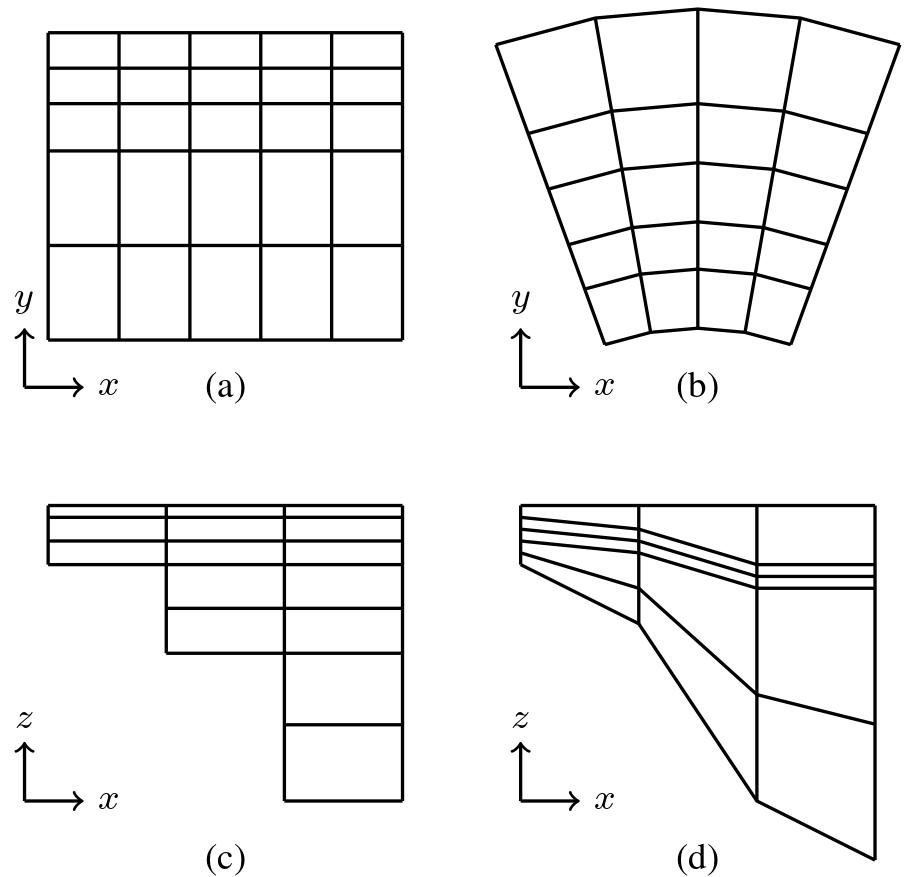
\includegraphics[width=7cm]{contents/grid.jpg}
		\caption{Diskritisasi grid dalam Parcels. Di bidang horizontal: (a) grid persegi, (b) grid lengkung, di bidang vertikal: (c) grid level z, (d) grid level s \protect\shortcite{Delandmeter2019}}.
		\label{fig:grid}
	\end{figure}
	
	Dalam aplikasinya, Parcels mengimplementasikan grid bertingkat (\textit{staggered grid}) yang diperkenalkan oleh \shortciteNP{ARAKAWA1977}, yaitu grid A, B dan C. Lebih lanjut, antara grid A, dan grid C terdapat perbedaan fundamental yaitu letak penyimpanan simpul variabel (lihat Gambar \ref{fig:arakawa}), sedangkan grid B dapat dianggap sebagai peralihan dari grid A ke grid C dan perbedaan tipe model grid ini menjadi penting dikarenakan peningkatan kapasitas komputasi yang stabil di banyak pusat pemodelan iklim telah mengantarkan periode transisi untuk model laut global  \shortcite{Barham2018,Delandmeter2019}. Visualisasi diskritisasi pada C-grid Arakawa yang lebih lengkap dapat dilihat dalam Gambar \ref{fig:arakawa_1}-\ref{fig:arakawa_5} pada Lampiran 2.
	
	\begin{figure}[H]
		\centering
		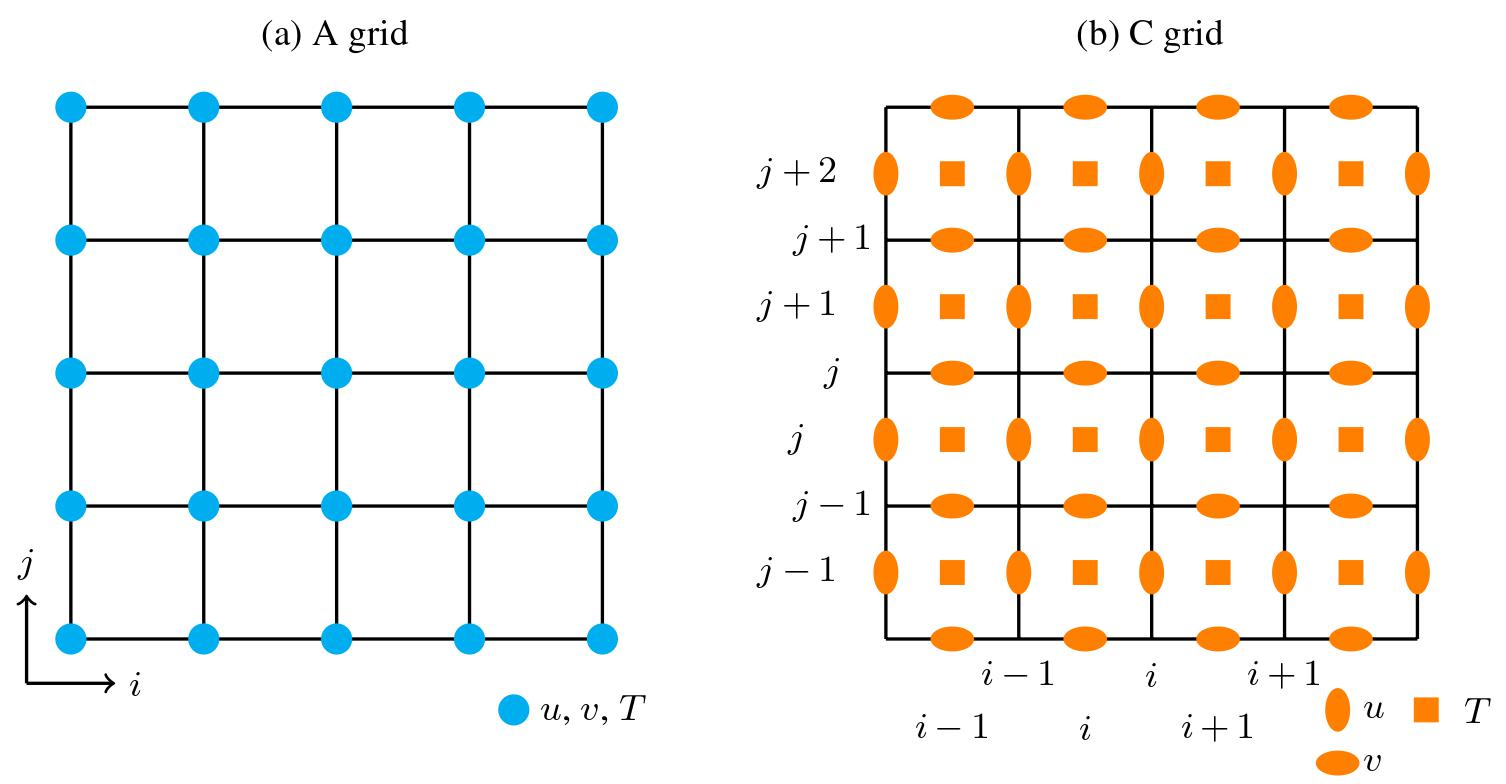
\includegraphics[width=13cm]{contents/arakawa.jpg}
		\caption{Grid Arakawa: (a) Grid A dan (b) Grid C \protect\shortcite{Delandmeter2019}}
		\label{fig:arakawa}
		\medspace
		\small
		Grid A adalah satu-satunya \textit{unstaggered grid} dalam grid Arakawa dimana variabel-variabelnya (\textit{zonal velocity (u), meridional velocity (v), tracers (T)}) hanya terdapat pada titik sudut grid, berbeda dengan grid C yang berada di sisi dan tengah grid. $i$ dan $j$ adalah indeks yang merepresentasikan variabel kolom dan baris dimana variabel disimpan.
	\end{figure}
	Selanjutnya, akan dijabarkan skema interpolasi yang diimplementasikan dalam Parcels untuk \textit{curvelinear} C-grid Arakawa pada bidang 2-D dan 3-D.

\subsection[Bidang 2-D]{Bidang 2-D}
	Definisikan fungsi $f$ sebagai suatu bidang yang diinterpolasi dalam sel $(i,j)$ dengan polinomial Lagrange $\phi_n^{2-D}$ dan 4 titik sentral $F_n, n=0...3$ yang mengelilingi sel, sehingga
	\begin{equation}
		f(x,y)=\sum_{n=0}^{3}\phi_n^{2-D}(\xi,\eta)F_n, 
	\end{equation}
	dengan $\psi, \eta$ memenuhi  
	\begin{equation}\label{eq:xy_2d}
		\begin{cases}
			x &= \sum_n \phi_n^{2-D}(\xi,\eta)X_n \\
			y &= \sum_n \phi_n^{2-D}(\xi,\eta)Y_n.
		\end{cases}	
	\end{equation}
	Polinomial Langrange 2-D didasarkan atas polinomial Lagrange 1-D dan memiliki bentuk umum \shortcite{Bozorgmanesh2009}:
	\begin{equation*}
		\begin{aligned}
			\phi_{ij} = \phi_i (x) \phi_j (y), \quad 0 \leq i \leq n, 0 \leq j \leq m \\
			\phi_i (x) = \prod_{s=0,s\neq i}^n \left(\frac{x-x_s}{x_i-x_s}\right), \quad \phi_j (y) = \prod_{s=0,s\neq i}^m \left(\frac{y-y_s}{y_i-y_s}\right) \\	
		\end{aligned}
	\end{equation*}
	sehingga diperoleh, 
	\begin{equation*}
		\phi_i (x) \phi_j (y) = \phi_{ij} (x_r,y_r)=
		\begin{cases}
			1	\quad	i=r,\;j=s \\
			0	\quad	\text{lainnya}
		\end{cases}
	\end{equation*}
	Polinomial Lagrange 2-D $\phi_n^{2-D}$ untuk $n=0,1,2,3$ menjadi
	\begin{equation*}
		\begin{aligned}
			\phi_0^{2-D} &= (1-\xi)(1-\eta), \quad 	\phi_1^{2-D} &= \xi(1-\eta) \\
			\phi_2^{2-D} &= \xi\eta, \quad 	\quad \quad \quad \quad \quad \phi_3^{2-D} &= (1-\xi)\eta.
		\end{aligned}
	\end{equation*}
	Perhatikan bahwa kecepatan relatif $\xi,\text{dan}\;\eta$ untuk grid A (grid persegi) dapat dengan mudah dicari dengan menyelesaikan persamaan \ref{eq:xy_2d} dan mengingat hubungan $X_0=X_3,X_1=X_2,Y_0=Y_1,\text{dan} \;Y_2=Y_3$, diperoleh  
	\begin{equation*}
		\begin{aligned}
			x &= \phi_0 X_0 + \phi_1 X_1 + \phi_2 X_2 + \phi_3 X_3 \\
			&= (1-\xi)(1-\eta)X_0+\xi(1-\eta)X_1+\xi\eta X_1 +(1-\xi)\eta X_0 \\
			&= X_0 + \xi\eta X_0 - \xi X_0 - \eta X_0 + \xi X_1 - \xi\eta X_1 + \xi\eta X_1 + \eta X_0 - \xi\eta X_0 \\
			&= X_0 - \xi X_0 + \xi X_1 \\
			\therefore \xi &= \frac{x-X_0}{X_1-X_0}. \\
			y &= \phi_0 Y_0 + \phi_1 Y_1 + \phi_2 Y_2 + \phi_3 Y_3 \\
			&= (1-\xi)(1-\eta)Y_0+\xi(1-\eta)Y_0+\xi\eta Y_3 +(1-\xi)\eta Y_3 \\
			&= Y_0 - \xi Y_0 - \eta Y_0 + \xi\eta Y_0 + \xi Y_0 - \xi\eta Y_0 + \xi\eta Y_3 + \eta Y_3 - \xi\eta Y_3 \\
			&= Y_0 - \eta Y_0 + \eta Y_3\\
			\therefore \eta &= \frac{y-Y_0}{Y_3-Y_0}. 
		\end{aligned}
	\end{equation*}
	\begin{figure}[H]
		\centering
		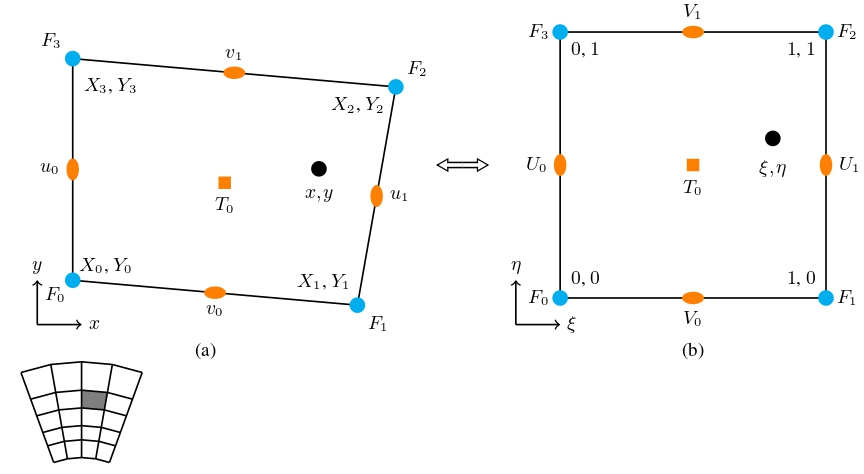
\includegraphics[width=13cm]{contents/mesh_arakawa.jpg}
		\caption{Posisi variabel pada grid A (titik biru), dan grid C (titik jingga) dengan (a) koordinat fisik dalam sel jala (\textit{mesh cell}), (b) koordinat relatif dalam sel satuan (\textit{unit cell}) \protect\shortcite{Delandmeter2019}}
		\label{fig:mesh}
	\end{figure}
	Komponen kecepatan dari Gambar \ref{fig:arakawa}b dapat ditulis menjadi $(u_0=u_{j+1,i}, u_1=u_{j+1,i+1}, v_0=v_{j,i+1}, v_1=v_{j+1,i+1})$ dan digambarkan sedemikian sebagai Gambar \ref{fig:mesh}a. Kemudian kecepatan pada posisi $(x,y)$ didekati dengan interpolasi linear fluks $(U_0,U_1,V_0,V_1)$ pada sisi-sisi sel (Gambar \ref{fig:mesh}b) sehingga
	\begin{equation}\label{eq:linearflux}
		\begin{cases}
			U_0	= L_{03} u_0, \\
			U_1	= L_{12} u_1, \\
			V_0	= L_{01} v_0, \\
			V_1	= L_{23} v_1, 
		\end{cases}
	\end{equation}
	dengan $L_{03},L_{12},L_{01},\text{dan}\;L_{23}$ adalah panjang sisi sel. Selanjutnya dengan menggunakan persamaan \ref{eq:xy_2d}, misalkan matriks Jacobian 2-D yang mentransformasikan sel fisik menjadi sel satuan pada Gambar \ref{fig:mesh} yang didefinisikan sebagai
	\begin{equation*}
		\textbf{J}^{2-D}(\xi,\eta)=
		\begin{bmatrix}
			\frac{\partial x}{\partial \xi} & \frac{\partial x}{\partial \eta}\\
			\frac{\partial y}{\partial \xi} & \frac{\partial y}{\partial \eta}
		\end{bmatrix}
		=
		\begin{bmatrix}
			\sum_n\frac{\partial \phi_n^{2-D}}{\partial \xi}X_n & \sum_n\frac{\partial \phi_n^{2-D}}{\partial \eta}X_n\\
			\sum_n\frac{\partial y}{\partial \phi_n^{2-D}}Y_n & \sum_n\frac{\partial \phi_n^{2-D}}{\partial \eta}Y_n 
		\end{bmatrix}
	\end{equation*}
	\begin{equation}\label{eq:jacob_2d}
		= \left(\sum_n\frac{\partial \phi_n^{2-D}}{\partial \xi}X_n\right)\left(\sum_n\frac{\partial \phi_n^{2-D}}{\partial \eta}Y_n\right)-\left(\sum_n\frac{\partial \phi_n^{2-D}}{\partial \eta}X_n\right) \left(\sum_n\frac{\partial y}{\partial \phi_n^{2-D}}Y_n \right).
	\end{equation}

	Determinan dari matriks Jacobian pada persamaan \ref{eq:jacob_2d} selanjutnya dinotasikan $J^{2-D}(\xi,\eta)=\text{det}(\textbf{J}^{2-D})$ dan didefinisikan sebagai rasio antara permukaan dasar dalam sel fisik dan permukaan yang bersesuaian dalam sel satuan. Kecepatan relatif dalam sel satuan didefinisikan sebagai
	\begin{equation}
		\begin{cases}
			\frac{\partial \xi}{\partial t} &= \frac{(1-\xi)U_0+\xi U_1}{J^{2-D}(\xi,\eta)}, \\
			\frac{\partial \eta}{\partial t} &= \frac{(1-\eta)V_0+\eta V_1}{J^{2-D}(\xi,\eta)}.
		\end{cases}	
	\end{equation}
	Dengan mentransformasikan kecepatan relatif kedalam sistem koordinat fisik diperoleh,
	\begin{equation*}
		\begin{aligned}
			u &= \frac{\partial x}{\partial t} = \sum_n \left(\frac{\partial \phi_n^{2-D}}{\partial \xi}\frac{\partial \xi}{\partial t}+\frac{\partial \phi_n^{2-D}}{\partial \eta}\frac{\partial \eta}{\partial t}\right)X_n \\
			&= \sum_n \left(\frac{\partial \phi_n^{2-D}}{\partial \xi}\frac{\partial \xi}{\partial t}\right)X_n + \sum_n \left(\frac{\partial \phi_n^{2-D}}{\partial \eta}\frac{\partial \eta}{\partial t}\right)X_n \\
			&= \sum_n \left(\frac{\partial \phi_n^{2-D}}{\partial \xi}X_n\right)\frac{\partial \xi}{\partial t} + \sum_n \left(\frac{\partial \phi_n^{2-D}}{\partial \eta}X_n\right)\frac{\partial \eta}{\partial t} \\
			&= \frac{\partial x}{\partial \xi}\frac{\partial \xi}{\partial t}+\frac{\partial x}{\partial \eta}\frac{\partial \eta}{\partial t}, \\
			v &= \frac{\partial y}{\partial t} = \sum_n \left(\frac{\partial \phi_n^{2-D}}{\partial \xi}\frac{\partial \xi}{\partial t}+\frac{\partial \phi_n^{2-D}}{\partial \eta}\frac{\partial \eta}{\partial t}\right)Y_n \\
			&= \sum_n \left(\frac{\partial \phi_n^{2-D}}{\partial \xi}\frac{\partial \xi}{\partial t}\right)Y_n + \sum_n \left(\frac{\partial \phi_n^{2-D}}{\partial \eta}\frac{\partial \eta}{\partial t}\right)Y_n \\
			&= \sum_n \left(\frac{\partial \phi_n^{2-D}}{\partial \xi}Y_n\right)\frac{\partial \xi}{\partial t} + \sum_n \left(\frac{\partial \phi_n^{2-D}}{\partial \eta}Y_n\right)\frac{\partial \eta}{\partial t} \\
			&= \frac{\partial y}{\partial \xi}\frac{\partial \xi}{\partial t}+\frac{\partial y}{\partial \eta}\frac{\partial \eta}{\partial t}.
		\end{aligned}	
	\end{equation*}
\subsection[Ruang 3-D]{Ruang 3-D}
	Skema interpolasi ruang 3-D digunakan untuk mendiskritisasi grid di bidang vertikal yaitu koordinat z (\ref{fig:grid}c) dan koordinat s (\ref{fig:grid}d), dan memiliki 8 titik sentral pada titik simpul hexahedron (Gambar \ref{fig:mesh3d}). Polinomial Lagrange 3-D $\phi_n^{3-D}$ untuk $n = 0,1,\dots,7$ berbentuk
	\begin{equation*}
		\begin{aligned}
			\begin{matrix}
				\phi_0^{3-D} =& (1-\xi)(1-\eta)(1-\zeta), & \phi_4^{3-D} =& (1-\xi)(1-\eta)\zeta, \\
				\phi_1^{3-D} =& \xi(1-\eta)(1-\zeta),  & \phi_5^{3-D} =& \xi(1-\eta)\zeta, \\
				\phi_2^{3-D} =& \xi \eta(1-\zeta),  & \phi_6^{3-D} =& \xi\eta\zeta, \\
				\phi_3^{3-D} =& (1-\xi)\eta(1-\zeta),  & \phi_7^{3-D} =& (1-\xi)\eta\zeta.
			\end{matrix}
		\end{aligned}
	\end{equation*}
	Apabila persamaan \ref{eq:xy_2d} diperluas menjadi 3-D maka akan berbentuk
	\begin{equation}\label{eq:xyz_3d}
		\begin{cases}
			x = \sum_n \phi_{n}^{3-D}(\xi,\eta,\zeta)X_n,\\
			y = \sum_n \phi_{n}^{3-D}(\xi,\eta,\zeta)Y_n,\\
			z = \sum_n \phi_{n}^{3-D}(\xi,\eta,\zeta)Z_n.
		\end{cases}		
	\end{equation}
	Selesaikan persamaan \ref{eq:xyz_3d}c dengan menggunakan polinomial Lagrange 3-D, diperoleh kecepatan relatif
	\begin{equation}\label{eq:zeta_velo}
		\begin{aligned}
			\zeta = \frac{z-z_0}{z_1-z_0},
		\end{aligned}
	\end{equation}
	dengan 
	\begin{equation*}
		\begin{cases}
			z_0 = \sum_{n=0}^{3}\phi_n^{3-D}Z_n, \\
			z_1 = \sum_{n=4}^{7}\phi_n^{3-D}Z_n.
		\end{cases}
	\end{equation*}
	\begin{figure}[H]
		\centering
		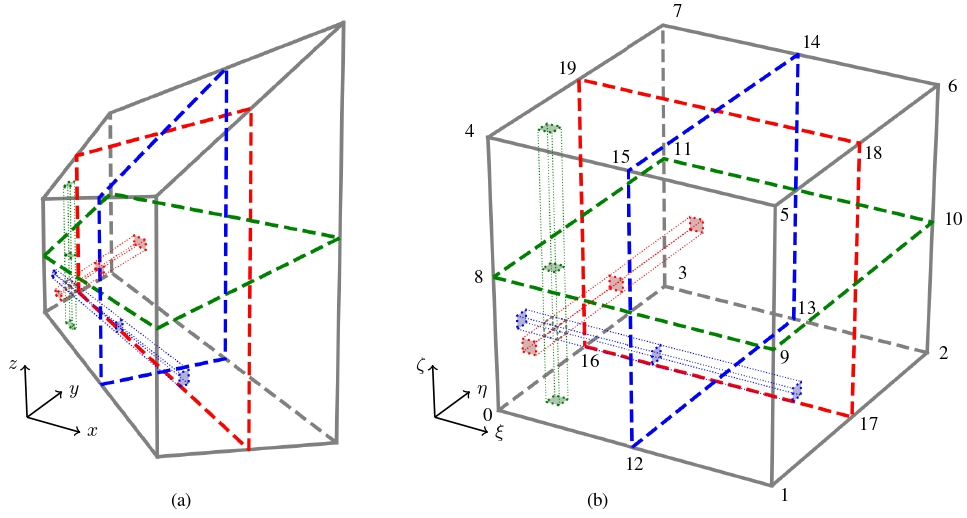
\includegraphics[width=13cm]{contents/mesh_arakawa3d.jpg}
		\caption{Fluks yang digunakan untuk interpolasi 3-D pada grid C Arakawa: (a) sel fisik, (b) sel satuan \protect\shortcite{Delandmeter2019}}
		\label{fig:mesh3d}
	\end{figure}
	Selanjutnya, perlu dicatat bahwa interpolasi pada grid C Arakawa berbeda untuk koordinat z dan koordinat s. Pada koordinat z, arah horizontal dan vertikal berbeda. Untuk sel $(k,j,i)$, kecepatan horizontal diinterpolasi seperti dalam kasus 2-D dengan menggunakan data $k:(U_{k,j+1,i},U_{k,j+1,i+1},V_{k,j,i+1},V_{k,j+1,i+1})$, tetapi untuk kecepatan vertikal diinterpolasi seperti dalam persamaan \ref{eq:zeta_velo}, yaitu
	\begin{equation}
		w = \zeta w_0 + (1-\zeta)w_1,
	\end{equation}
	dengan $w_0=w_{k,j+1,i+1}$ dan $w_1=w_{k+1,j+1,i+1}$.
	Untuk koordinat s, tiga kecepatan $(u,v,\text{dan}\;w)$ harus diinterpolasi sekaligus seperti halnya dalam bidang 2-D. Misalkan matriks Jacobian 3-D untuk koordinat $\xi,\eta,\text{dan}\; \zeta$ sebagai
	\begin{equation*}
		\textbf{J}^{3-D}(\xi,\eta,\zeta)=
		\begin{bmatrix}
			\frac{\partial x}{\partial \xi} & \frac{\partial x}{\partial \eta} & \frac{\partial x}{\partial \zeta}\\
			\frac{\partial y}{\partial \xi} & \frac{\partial y}{\partial \eta} & \frac{\partial y}{\partial \zeta}\\
			\frac{\partial z}{\partial \xi} & \frac{\partial z}{\partial \eta} & \frac{\partial z}{\partial \zeta}
		\end{bmatrix}
		=
		\begin{bmatrix}
			\sum_n\frac{\partial \phi_n^{3-D}}{\partial \xi}X_n & \sum_n\frac{\partial \phi_n^{3-D}}{\partial \eta}X_n & \sum_n\frac{\partial \phi_n^{3-D}}{\partial \zeta}X_n\\
			\sum_n\frac{\partial \phi_n^{3-D}}{\partial \phi_n^{3-D}}Y_n & \sum_n\frac{\partial \phi_n^{3-D}}{\partial \eta}Y_n & \sum_n\frac{\partial \phi_n^{3-D}}{\partial \zeta}Y_n \\
			\sum_n\frac{\partial \phi_n^{3-D}}{\partial \phi_n^{3-D}}Z_n & \sum_n\frac{\partial \phi_n^{3-D}}{\partial \eta}Z_n & \sum_n\frac{\partial \phi_n^{3-D}}{\partial \zeta}Z_n
		\end{bmatrix}.
	\end{equation*}
	Notasikan determinan dari matriks Jacobian sebagai $J^{3-D}(\xi,\eta,\zeta)=\text{det}(\textbf{J}^{3-D})$. Berbeda dengan 2-D, untuk 3-D kecepatan relatif diinterpolasi dengan menggunakan fungsi Lagrangian kuadratik, yaitu
	\begin{equation}
		\begin{cases}
			\frac{\partial \xi}{\partial t}&=\frac{(2\xi^2-3\xi+1)U_0+(-4\xi^2+4\xi)U_\frac{1}{2}+(2\xi^2-\xi)U_1}{J^{3-D}(\xi,\eta,\zeta)},\\
			\frac{\partial \eta}{\partial t}&=\frac{(2\eta^2-3\eta+1)U_0+(-4\eta^2+4\eta)U_\frac{1}{2}+(2\eta^2-\eta)U_1}{J^{3-D}(\xi,\eta,\zeta)},\\
			\frac{\partial \zeta}{\partial t}&=\frac{(2\zeta^2-3\zeta+1)U_0+(-4\zeta^2+4\zeta)U_\frac{1}{2}+(2\zeta^2-\zeta)U_1}{J^{3-D}(\xi,\eta,\zeta)}.
		\end{cases}
	\end{equation}
	Dengan mentransformasikan kecepatan relatif kedalam sistem koordinat fisik menggunakan persamaan \ref{eq:xyz_3d} diperoleh,
	\begin{equation*}
		\begin{aligned}
			u &= \frac{\partial x}{\partial t} = \sum_n \left(\frac{\partial \phi_n^{3-D}}{\partial \xi}\frac{\partial \xi}{\partial t}+\frac{\partial \phi_n^{3-D}}{\partial \eta}\frac{\partial \eta}{\partial t}+\frac{\partial \phi_n^{3-D}}{\partial \zeta}\frac{\partial \zeta}{\partial t}\right)X_n \\
			&= \sum_n \left(\frac{\partial \phi_n^{3-D}}{\partial \xi}\frac{\partial \xi}{\partial t}\right)X_n + \sum_n \left(\frac{\partial \phi_n^{3-D}}{\partial \eta}\frac{\partial \eta}{\partial t}\right)X_n + \sum_n \left(\frac{\partial \phi_n^{3-D}}{\partial \zeta}\frac{\partial \zeta}{\partial t}\right)X_n \\
			&= \sum_n \left(\frac{\partial \phi_n^{3-D}}{\partial \xi}X_n\right)\frac{\partial \xi}{\partial t} + \sum_n \left(\frac{\partial \phi_n^{3-D}}{\partial \eta}X_n\right)\frac{\partial \eta}{\partial t} + \sum_n \left(\frac{\partial \phi_n^{3-D}}{\partial \zeta}X_n\right)\frac{\partial \zeta}{\partial t}\\
			&= \frac{\partial x}{\partial \xi}\frac{\partial \xi}{\partial t}+\frac{\partial x}{\partial \eta}\frac{\partial \eta}{\partial t}+\frac{\partial x}{\partial \zeta}\frac{\partial \zeta}{\partial t}, \\
			v &= \frac{\partial t}{\partial t} = \sum_n \left(\frac{\partial \phi_n^{3-D}}{\partial \xi}\frac{\partial \xi}{\partial t}+\frac{\partial \phi_n^{3-D}}{\partial \eta}\frac{\partial \eta}{\partial t}+\frac{\partial \phi_n^{3-D}}{\partial \zeta}\frac{\partial \zeta}{\partial t}\right)Y_n \\
			&= \sum_n \left(\frac{\partial \phi_n^{3-D}}{\partial \xi}\frac{\partial \xi}{\partial t}\right)Y_n + \sum_n \left(\frac{\partial \phi_n^{3-D}}{\partial \eta}\frac{\partial \eta}{\partial t}\right)Y_n + \sum_n \left(\frac{\partial \phi_n^{3-D}}{\partial \zeta}\frac{\partial \zeta}{\partial t}\right)Y_n \\
			&= \sum_n \left(\frac{\partial \phi_n^{3-D}}{\partial \xi}Y_n\right)\frac{\partial \xi}{\partial t} + \sum_n \left(\frac{\partial \phi_n^{3-D}}{\partial \eta}Y_n\right)\frac{\partial \eta}{\partial t}+ \sum_n \left(\frac{\partial \phi_n^{3-D}}{\partial \zeta}Y_n\right)\frac{\partial \zeta}{\partial t}\\
			&= \frac{\partial y}{\partial \xi}\frac{\partial \xi}{\partial t}+\frac{\partial y}{\partial \eta}\frac{\partial \eta}{\partial t}+\frac{\partial y}{\partial \zeta}\frac{\partial \zeta}{\partial t}, \\
			w &= \frac{\partial t}{\partial t} = \sum_n \left(\frac{\partial \phi_n^{3-D}}{\partial \xi}\frac{\partial \xi}{\partial t}+\frac{\partial \phi_n^{3-D}}{\partial \eta}\frac{\partial \eta}{\partial t}+\frac{\partial \phi_n^{3-D}}{\partial \zeta}\frac{\partial \zeta}{\partial t}\right)Z_n \\
			&= \sum_n \left(\frac{\partial \phi_n^{3-D}}{\partial \xi}\frac{\partial \xi}{\partial t}\right)Z_n + \sum_n \left(\frac{\partial \phi_n^{3-D}}{\partial \eta}\frac{\partial \eta}{\partial t}\right)Z_n + \sum_n \left(\frac{\partial \phi_n^{3-D}}{\partial \zeta}\frac{\partial \zeta}{\partial t}\right)Z_n \\
			&= \sum_n \left(\frac{\partial \phi_n^{3-D}}{\partial \xi}Z_n\right)\frac{\partial \xi}{\partial t} + \sum_n \left(\frac{\partial \phi_n^{3-D}}{\partial \eta}Z_n\right)\frac{\partial \eta}{\partial t}+ \sum_n \left(\frac{\partial \phi_n^{3-D}}{\partial \zeta}Z_n\right)\frac{\partial \zeta}{\partial t}\\
			&= \frac{\partial z}{\partial \xi}\frac{\partial \xi}{\partial t}+\frac{\partial z}{\partial \eta}\frac{\partial \eta}{\partial t}+\frac{\partial z}{\partial \zeta}\frac{\partial \zeta}{\partial t}.
		\end{aligned}	
	\end{equation*}
	Untuk menghitung nilai fluks pada sel satuan, tidak seperti pendekatan pada persamaan \ref{eq:linearflux} dengan koordinat $\xi \; \text{dan} \; \eta$ saling bebas, fluks diinterpolasi sebagai perkalian kecepatan dengan muka Jacobian yang dinotasikan dengan $J_i^{2-D,f}$ dan didefinisikan sebagai 
	\begin{equation}
		J_i^{2-D,f}(\xi,\eta,\zeta)=\sqrt{(M_{0,i}(\textbf{J}^{3-D}))^2+(M_{1,i}(\textbf{J}^{3-D}))^2+(M_{2,i}(\textbf{J}^{3-D}))^2},
	\end{equation}
	dengan $M_{j,i}(\textbf{J}^{3-D}),\; j,i \; \text{minor dari}\; \textbf{J}^{3-D}$ dengan kata lain determinan dari matriks Jacobian $\textbf{J}^{3-D}$ dimana baris j dan kolom i dihilangkan, menghasilkan matriks $2\times2$. Akibatnya, Jacobian menjadi suatu fungsi dari koordinat-koordinat yang bersesuaian. Hal ini dikarenakan antarmuka pada Gambar \ref{fig:mesh3d} tidak akan terdistorsi secara merata dari sel fisik ke sel satuan. Lebih lanjut, flux normal terhadap $\xi,\eta,\; \text{atau}\; \zeta$ dalam sel satuan (lihat Gambar \ref{fig:mesh3d}b) dihitung dengan Jacobian $J_0^{2-D,f},J_1^{2-D,f},J_2^{2-D,f}$ sehingga diperoleh nilai-nilai pada Tabel \ref{table:flux_interp}.
	\begin{table}[htp]
	\centering
	\caption{Nilai Jacobian dan flux}
	\label{table:flux_interp}
		\begin{tabular}{lll}
			Face & Jacobian & Flux \\ \hline
			$[0,3,7,4]$ & $J_0^{2-D,f}(0,\eta,\zeta)$ & $U_0=u_0 J_0^{2-D,f}(0,\eta,\zeta)$ \\
			$[1,2,6,5]$ & $J_0^{2-D,f}(1,\eta,\zeta)$ & $U_1=u_1 J_0^{2-D,f}(1,\eta,\zeta)$  \\
			$[12,13,14,15]$ & $J_0^{2-D,f}(\frac{1}{2},\eta,\zeta)$ & $U_\frac{1}{2}=u_\frac{1}{2} J_0^{2-D,f}(\frac{1}{2},\eta,\zeta)$  \\
			$[0,1,5,4]$ & $J_1^{2-D,f}(\xi,0,\zeta)$ & $V_0=v_0 J_1^{2-D,f}(\xi,0,\zeta)$  \\
			$[3,2,6,7]$ & $J_1^{2-D,f}(\xi,1,\zeta)$ & $V_1=v_1 J_1^{2-D,f}(\xi,1,\zeta)$  \\
			$[16,17,18,19]$ & $J_1^{2-D,f}(\xi,\frac{1}{2},\zeta)$ & $V_\frac{1}{2}=v_\frac{1}{2} J_1^{2-D,f}(\xi,\frac{1}{2},\zeta)$  \\
			$[0,1,2,3]$ & $J_2^{2-D,f}(\xi,\eta,0)$ & $W_0=w_0 J_2^{2-D,f}(\xi,\eta,0)$  \\
			$[4,5,6,7]$ & $J_2^{2-D,f}(\xi,\eta,1)$ & $W_1=w_1 J_2^{2-D,f}(\xi,\eta,1)$  \\
			$[8,9,10,11]$ & $J_2^{2-D,f}(\xi,\eta,\frac{1}{2})$ & $W_\frac{1}{2}=w_\frac{1}{2} J_2^{2-D,f}(\xi,\eta,\frac{1}{2})$ 
		\end{tabular}
	\end{table}
%	Nilai-nilai $u_0,u_1,v_0,v_1,w_0,\;\text{dan}\;w_1$ dapat diketahui dari grid, sedangkan untuk nilai $u_\frac{1}{2},v_\frac{1}{2},\;\text{dan}\;w_\frac{1}{2}$ dapat dihitung sebagai berikut. Untuk muka $[12,13,14,15]$ pada Gambar \ref{fig:mesh3d}b,
%	\begin{equation}
%		\begin{aligned}
%			U_\frac{1}{2}^{+} &= u_0 J_0^{*2-D,f}(0,\frac{1}{2},\frac{1}{2})+v_0J_1^{*2-D,f}(0,\frac{1}{2},\frac{1}{2}) \\
%			& -v_1 J_1^{*2-D,f}(\frac{1}{2},1,\frac{1}{2}) + w_0 J_2^{*2-D,f}(\frac{1}{2},\frac{1}{2},0) \\
%			& -w_1 J_2^{*2-D,f}(\frac{1}{2},\frac{1}{2},1).
%		\end{aligned}
%	\end{equation}
%	Nilai fluks $U_\frac{1}{2}$ dihitung dengan cara,
	
\end{spacing}
	
